\section{Proposal}

\begin{frame}
	\frametitle{Research plan}
	
	\vspace{0.5cm}
	
	My research plan for the next year will focus on:
	
	\vspace{0.15cm}
	
	\begin{enumerate}
		\item extending the designed method
			  \begin{itemize}
		  		  \item implementing the ability of determining also the identities of the tracked objects;
			  	  \item introducing a component for data association.
			  \end{itemize}
		\item starting to learn basic behaviors of the tracked objects
	\end{enumerate}
\end{frame}

\begin{frame}
	\frametitle{Future directions}
	
	\vspace{0.2cm}
	
	\begin{itemize}
		\item Tracking of individuals within a crowd using the PETS2009 dataset
		
		\vspace{-0.3cm}
		
		\begin{center}
			\begin{tikzpicture}
				\node at (0,0) [draw=black,ultra thick,inner sep=0pt] {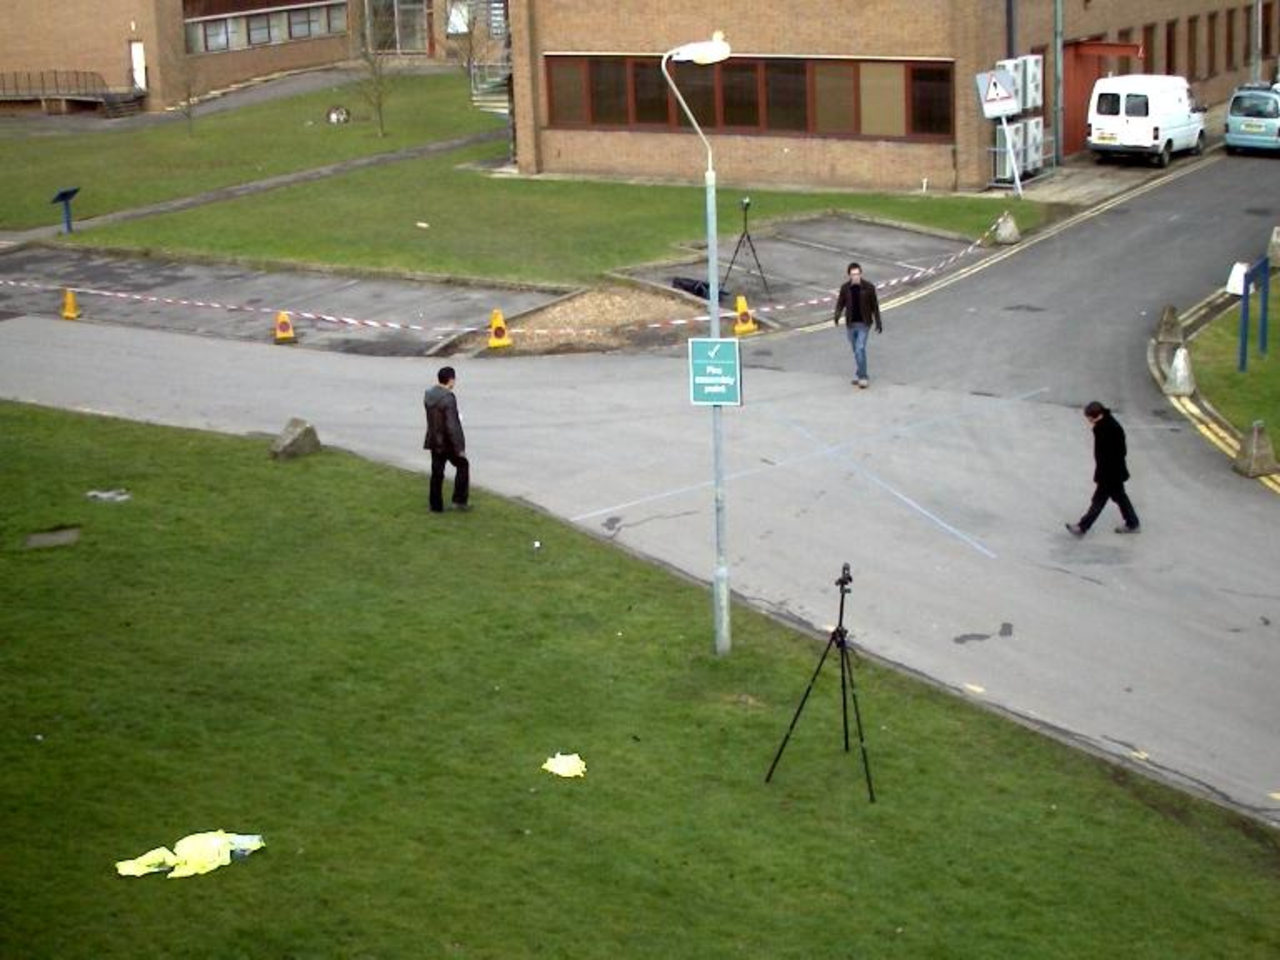
\includegraphics[scale=0.17]{images/Pets2009-1}};
				\node at (3.8,0) [draw=black,ultra thick,inner sep=0pt] {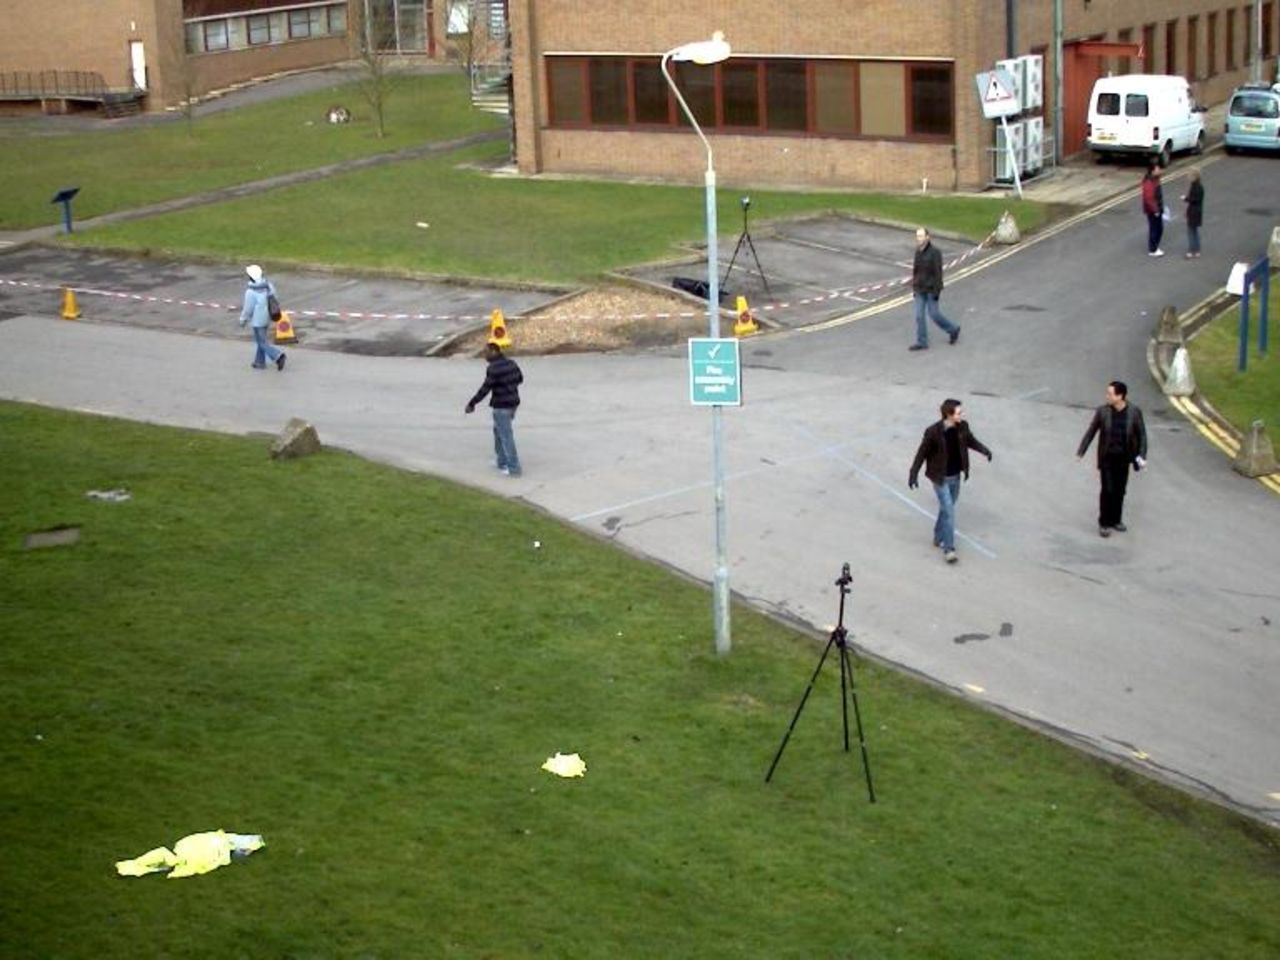
\includegraphics[scale=0.17]{images/Pets2009-2}};
				\node at (7.6,0) [draw=black,ultra thick,inner sep=0pt] {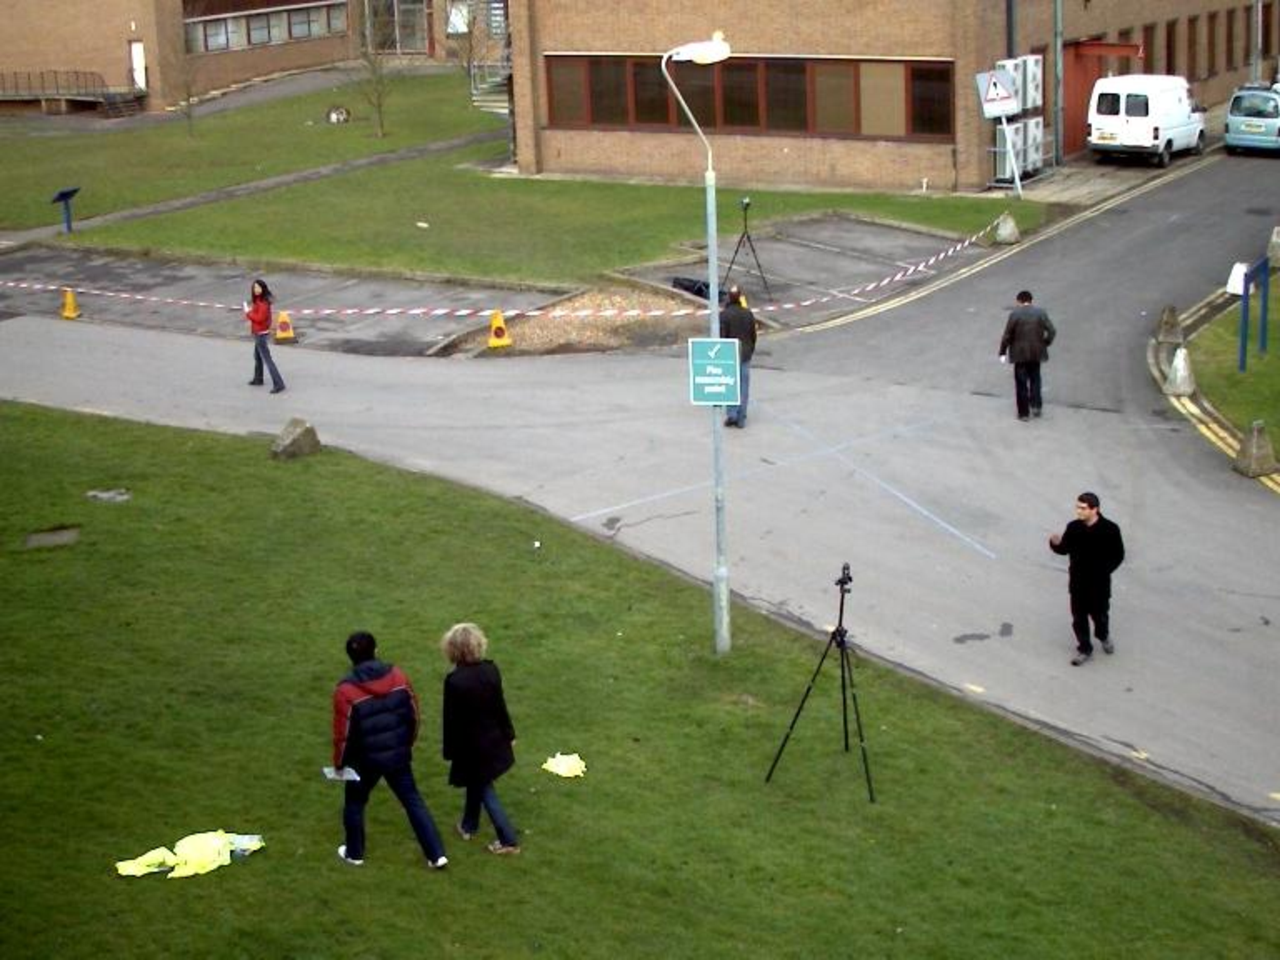
\includegraphics[scale=0.17]{images/Pets2009-3}};
			\end{tikzpicture}
		\end{center}
		
		\vspace{0.2cm}
		
		\item Ground-truth Acquisition of Humanoid Soccer Robot Behavior
		
		\vspace{0.08cm}
		
		\begin{center}
			\begin{tikzpicture}
				\node at (0,0) [draw=black,ultra thick,inner sep=0pt] {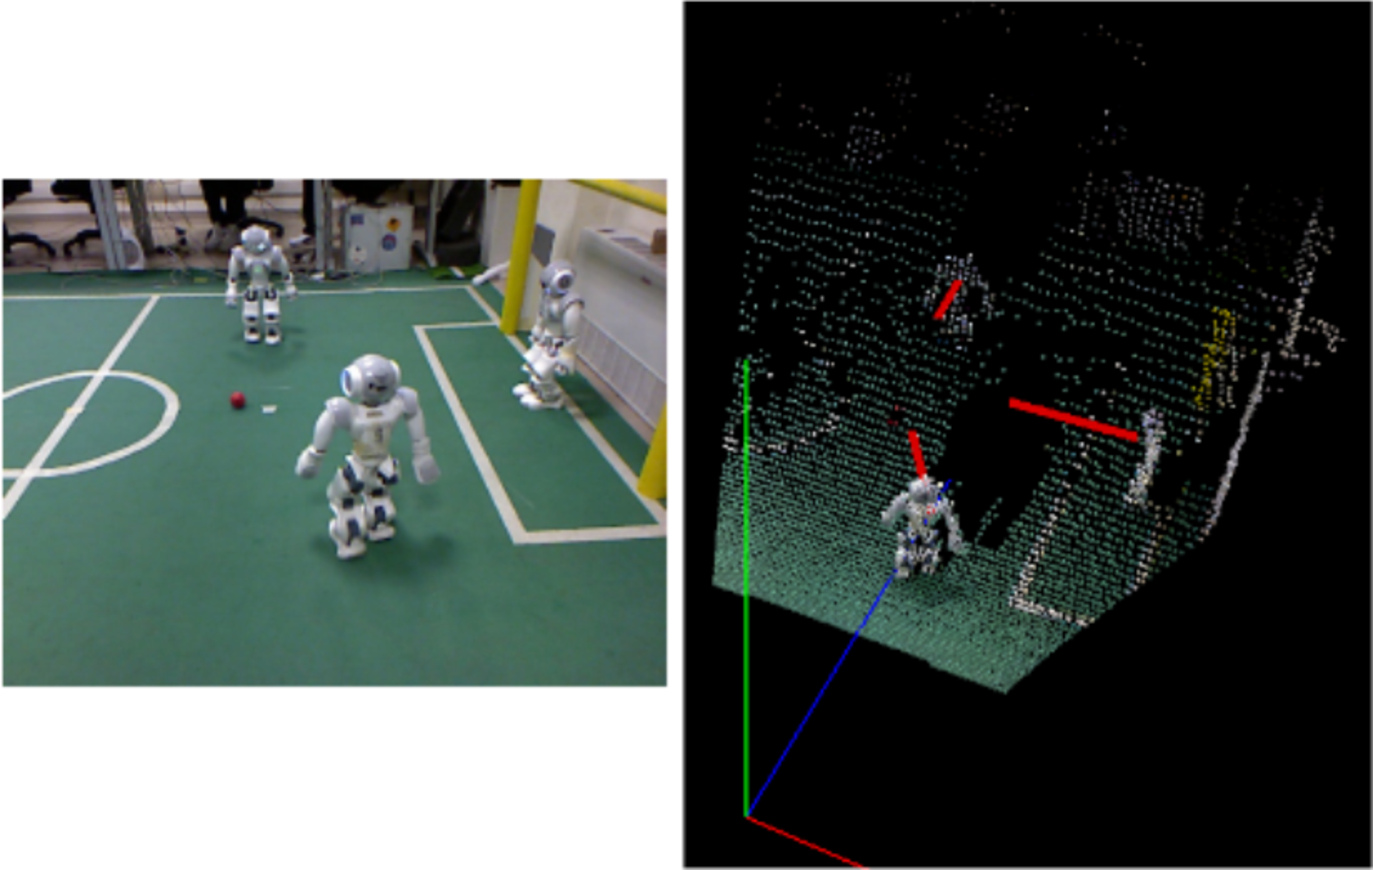
\includegraphics[scale=0.17]{images/GNAO}};
			\end{tikzpicture}
		\end{center}
	\end{itemize}
\end{frame}
